\chapter{主定理(主方法)}
\begin{introduction}
	\item 主定理的内容
	\item 主定理的用途
	\item 主定理的证明
\end{introduction}

\section{主定理的内容}
已知$T(n) = a T(\frac{n}{b}) + f(n)$,其中$a\geq 1, b\geq 1, f(n)$已知,则:
$$
\begin{array}{l}  
  \left\{\begin{matrix} 
  f(n) = O(n^{\log_{b}{a} - \epsilon} ),~T(n) = \Theta(n^{\log_{b}{a}} )  \\ 
  f(n) =  \Theta(n^{\log_{b}{a}} ),~T(n) = \Theta(n^{\log_{b}{a}}\log_{}{n} ) \\ 
  f(n) = \Omega (n^{\log_{b}{a} + \epsilon} ),T(n) = \Theta (f(n))
\end{matrix}\right.    
\end{array} 
$$
\section{主定理的用途}
        (1)\\
        $T(n)&=T\left(\frac{n}{2}\right)+\Theta(1)$\\
        $f(n)&=\Theta(1)=\Theta\left(n^{\log _{b} a}\right)=\Theta\left(n^{\log _{2} 1}\right)=\Theta(1)$\\
        $T(n)=\Theta\left(n^{\log _{2} 1} \log _{2} n\right)=\Theta\left(\log _{2} n\right)$\\\\
        ~~~(2)\\
        $T(n)=\Theta\left(n^{\log _{2} 1} \log _{2} n\right)=\Theta\left(\log _{2} n\right)T(n)=2 T\left(\frac{n}{2}\right)+\Theta(n)$\\
        $f(n)=\Theta(n)=\Theta\left(n^{\log _{b} a}\right)=\Theta\left(n^{\log _{2} 2}\right)=\Theta(n)$\\
        $T(n)=\Theta\left(n^{l o g_{2} 2} \log _{2} n=\Theta(n \log n)\right.$\\
\section{主定理的证明}
\subsection{假设 n 是 b 的整数次方}
\begin{figure}[htb]
	\centering
	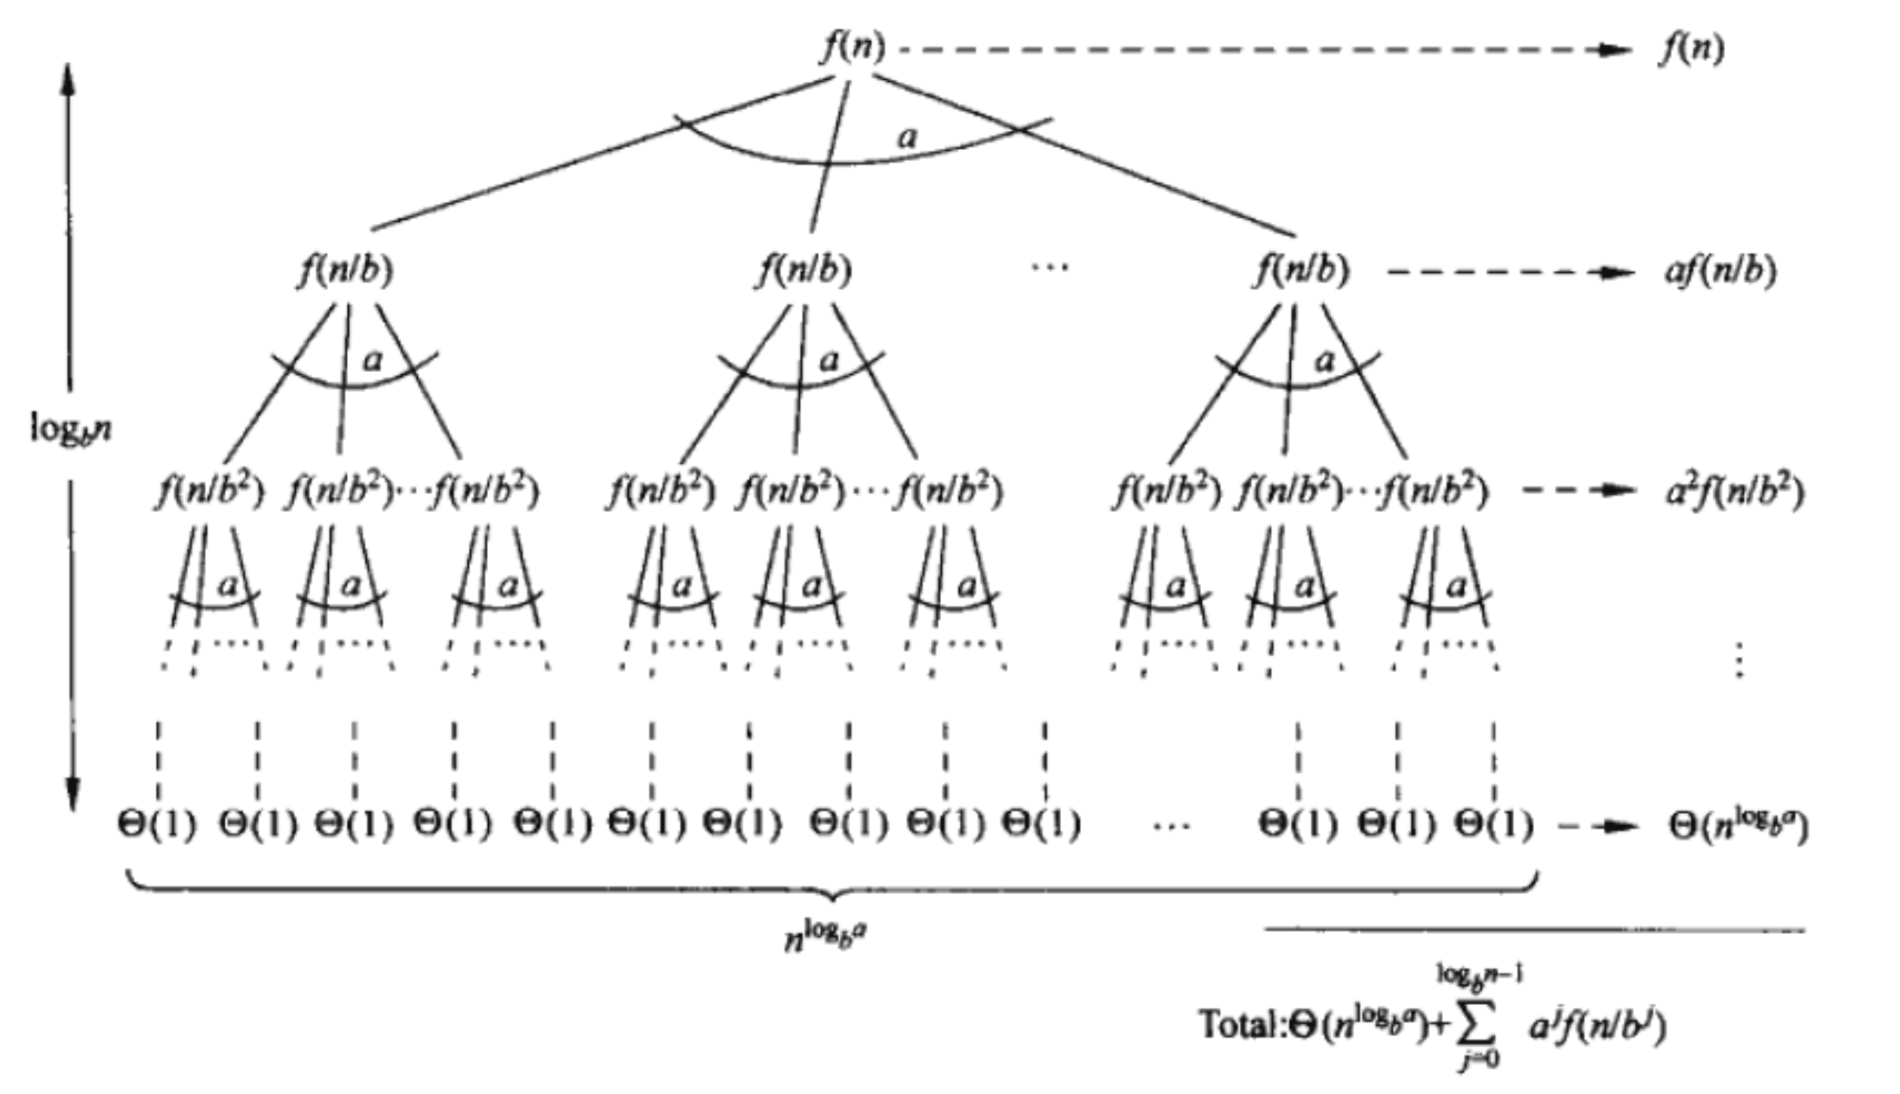
\includegraphics[scale=0.5]{image/mainmaster.png}
  \caption{递推式展开}\label{fig:nearestpoints-divide}
\end{figure}
 $T(n)=\Theta\left(n^{\log _{a} b}\right)+\sum_{j=0}^{\log _{b} n-1} a_{j} f\left(n / b^{j}\right)$\\
 (1)
 $$
 \begin{array}{l}
f(n)=O\left(n^{l o g_{b} a-\epsilon}\right) \\
g(n)=\sum_{j=0}^{\log _{b} n-1} a_{j} f\left(n / b^{j}\right) \\
f\left(n / b^{j}\right)=O\left(\left(\frac{n}{b^{j}}\right)^{\log _{b} a-\epsilon}\right) \\
c, n_{0}, \forall n \geq n_{0} \\
\left.f\left(n / b^{j}\right) \leq c\left(\frac{n}{b^{j}}\right)^{l o g_{b} a-\epsilon}\right) \Rightarrow a^{j} f\left(n / b^{j}\right) \leq c a^{j}\left(\frac{n}{b^{j}}\right)^{\log _{b} a-\epsilon} \\
a^{j} f\left(n / b^{j}\right) \leq c n^{\log _{b} a-\epsilon}\left(\frac{a}{b^{\log _{b} a-\epsilon}}\right)^{j} \\
\Rightarrow a^{j} f\left(n / b^{j}\right) \leq c n^{\log _{b} a-\epsilon}\left(\frac{a b^{\epsilon}}{b^{\log _{b} a}}\right)^{j} \\
\Rightarrow a^{j} f\left(n / b^{j}\right) \leq c n^{\log _{b} a-\epsilon}\left(b^{\epsilon}\right)^{j} \\
g(n) \leq c n^{\log _{b} a-\epsilon} \sum_{j=0}^{\log _{b} a-1}\left(b^{\epsilon}\right)^{j} \\
\Rightarrow \\g(n) \leq c n^{\log _{b} a-\epsilon} \frac{1\left(1-\left(b^{\epsilon}\right)^{l o g_{b} n}\right)}{1-b^{\epsilon}}
\Rightarrow g(n) \leq c n^{\log _{b} a-\epsilon \frac{1-n^{\epsilon}}{1-b^{\epsilon}}} \\
\Rightarrow g(n) \leq c \frac{n^{\log _{b} a-\epsilon}-n^{\log _{b} a}}{1-b^{\epsilon}} \\
g(n)=O\left(n^{\log _{b} a}\right) \\
T(n)=\Theta\left(n^{\log _{b} a}\right)+O\left(n^{\log _{b} a}\right)=\Theta\left(n^{\log _{b} a}\right)
\end{array}
 $$
(2)
$$
\begin{array}{l}
f(n)=\Theta\left(n^{\log _{b} a}\right) \\
g(n)=\sum_{j=0}^{\log _{b} n-1} a_{j} f\left(n / b^{j}\right) \\
f\left(n / b^{j}\right)=\Theta\left(\left(\frac{n}{b^{j}}\right)^{\log _{b} a}\right) \\
c_{1}, c_{2}, n_{0}, \forall n \geq n_{0} \\
c_{1}\left(\frac{n}{b^{j}}\right)^{l o g_{b} a} \leq f\left(n / b^{j}\right) \leq c_{2}\left(\frac{n}{b^{j}}\right)^{l o g_{b} a} \Rightarrow c_{1} a^{j}\left(\frac{n}{b^{j}}\right)^{l o g_{b} a} \leq a^{j} f\left(n / b^{j}\right) \leq c_{2} a^{j}\left(\frac{n}{b^{j}}\right)^{\log _{b} a} \\
c_{1} n^{\log _{b} a}\left(\frac{a}{b^{\log _{b} a}}\right)^{j} \leq a^{j} f\left(n / b^{j}\right) \leq c_{2} n^{\log _{b} a}\left(\frac{a}{b^{\log _{b} a}}\right)^{j} \\
\Rightarrow c_{1} n^{\log _{b} a} \leq a^{j} f\left(n / b^{j}\right) \leq c_{2} n^{\log _{b} a} \\
\Rightarrow c_{1} n^{\log _{b} a} \lg n \leq g(n) \leq c_{2} n^{\log _{b} a} \lg n \\
g(n)=\Theta\left(n^{\log _{b} a} \lg n\right)
\end{array}
$$
 

(3)

$$
\begin{array}{l}
f(n)=\Omega\left(n^{\log _{b} a+\epsilon}\right) \\
c<1 \text { af }\left(\frac{n}{b}\right) \leq c f(n) \\
g(n)=\sum_{j=0}^{\log _{b} n-1} a^{j} f\left(\frac{n}{b^{j}}\right) \\
a f\left(\frac{n}{b}\right) \leq c f(n) \\
\Rightarrow a^{j} f\left(\frac{n}{b^{j}}\right) \leq c^{j} f(n) \\
\Rightarrow g(n) \leq \sum_{j=0}^{\log _{b} n-1} c^{j} f(n) \\
\Rightarrow g(n) \leq \sum_{j=0}^{+\infty} c^{j} f(n)\\
\Rightarrow g(n) \leq \frac{1}{1-c} f(n) \\
g(n)=O(f(n))
\end{array}
$$

\subsection{假设 n 不是 b 的整数次方}
$T(n)=a T\left(\left\lfloor\frac{n}{b^{j}}\right\rfloor\right)+f(n) T(n)=a T\left(\left\lceil\frac{n}{b}\right\rceil\right)+f(n)$

$$
\begin{array}{c}
a^{\left\lfloor\log _{b} n\right\rfloor}<a^{\log _{b} n}<a * a^{\left\lfloor\log _{b} n\right\rfloor}, \\\quad \Theta\left(a^{\left\lfloor\log _{b} n\right\rfloor}\right)=\Theta\left(a^{\log _{b} n}\right)\\T(n)= 
\Theta\left(a^{\left\lfloor\log _{b} n\right\rfloor}\right)+\sum_{j=0}^{\left\lfloor\log _{b} n\right\rfloor-1} a^{j} f\left(n_{j}\right)\left(n_{j}=\left\lceil\frac{n}{b^{j}}\right\rceil\right) \\
\cdot \frac{n}{b^{j}} \leq \quad\left[\frac{n}{b^{j}}\right\rceil \quad<\quad \frac{n}{b^{j}}+1\\ \quad  \quad  \left\lceil\frac{n}{b^{j}}\right\rceil\left(\Theta\left(\frac{n}{b^{j}}\right)=\right. 
\left.\Theta\left(\left\lceil\frac{n}{b^{j}}\right\rceil\right)\right) 
\end{array}
$$

